\begin{itemize}
\tightlist
\item
  \protect\hyperlink{life-cycle-assessment}{Life Cycle Assessment}

  \begin{itemize}
  \tightlist
  \item
    \protect\hyperlink{basics-of-life-cycle-assessment}{Basics of Life
    Cycle Assessment}
  \item
    \protect\hyperlink{goal-and-scope-definition}{Goal and Scope
    definition}

    \begin{itemize}
    \tightlist
    \item
      \protect\hyperlink{goal}{Goal}
    \item
      \protect\hyperlink{scope}{Scope}
    \item
      \protect\hyperlink{system-boundaries}{System Boundaries}
    \end{itemize}
  \item
    \protect\hyperlink{the-basics-of-life-cycle-inventory}{The basics of
    life cycle inventory}

    \begin{itemize}
    \tightlist
    \item
      \protect\hyperlink{multi-functionality}{Multi-functionality}
    \end{itemize}
  \item
    \protect\hyperlink{marginal-vs-average}{Marginal vs Average}
  \item
    \protect\hyperlink{2-modelling-approaches}{2 modelling approaches}

    \begin{itemize}
    \tightlist
    \item
      \protect\hyperlink{modelling-context}{Modelling context}
    \item
      \protect\hyperlink{the-basics-of-life-cycle-impact-assessment}{The
      basics of life cycle impact assessment}
    \item
      \protect\hyperlink{interpretation}{Interpretation}
    \end{itemize}
  \item
    \protect\hyperlink{input-output-lca}{Input-output LCA}
  \end{itemize}
\item
  \protect\hyperlink{design-for-environment-dfe-methods-and-techniques}{Design
  for environment (DfE): Methods and Techniques}

  \begin{itemize}
  \tightlist
  \item
    \protect\hyperlink{product-concept-optimisation}{Product Concept
    Optimisation}
  \item
    \protect\hyperlink{material-selection}{Material Selection}
  \end{itemize}
\end{itemize}

\hypertarget{life-cycle-assessment}{%
\section{Life Cycle Assessment}\label{life-cycle-assessment}}

\hypertarget{basics-of-life-cycle-assessment}{%
\subsection{Basics of Life Cycle
Assessment}\label{basics-of-life-cycle-assessment}}

We need to quantize the impact human actions have on the environment.
This can be categorized in 3 main categories, namely :

\begin{enumerate}
\def\labelenumi{\arabic{enumi}.}
\tightlist
\item
  Ressource depletion
\item
  Ecosystem quality
\item
  Human health
\end{enumerate}

They are not easy to quantize but we can quantize the production and
equivalent production of certain molecules which have been proven to
have various effect on those 3 main issues.

\hypertarget{goal-and-scope-definition}{%
\subsection{Goal and Scope definition}\label{goal-and-scope-definition}}

\hypertarget{goal}{%
\subsubsection{Goal}\label{goal}}

Before any LCA, it is important to put boundaries and to explain to the
reader our goal and intended application. We need to specify the target
audience, be honest with our method (show its limitation), comparative
studies need to be showcased too and explicitly say the commissioner of
the study.

\hypertarget{scope}{%
\subsubsection{Scope}\label{scope}}

We need to set the \emph{functional unit} (primary goal or capacity
aimed) and also set clear system boundaries to properly take into
account the in and out.

We also need to indicate the principles for handling
\emph{multi-functionality}, LCIA impact categories, data quality
requirements, critical review needs. We often need high quality data to
have the best and most effective LCA.

\hypertarget{functional-unit}{%
\paragraph{Functional Unit}\label{functional-unit}}

It is a metric that represents the actual unity of a given product for a
given task (eg: \(m^2\) covered for a paint bucket, \(tons\) for a
crane, \ldots). It needs to set as a comparison and be equivalent
(comparing apple to apple).

Definition : \emph{The functional unit names and quantifies the
qualitative and quantitative aspects of the function(s) along the
questions ``what'', ``how much'', ``how well'', ``where'' and ``for how
long''. The functional unit must allow comparison between alternatives.}

Sometimes finding the right unit is quite tricky (eg: lamps) there is
many units that represents different use cases. We also need to notice
that the FU describes a \textbf{need} not a solution. Sometimes to be
more efficient we need to change the design and zoom out.

It is hard to be totally equivalent and to exactly build a perfect
metric for complex products. Often we won't have \textbf{complete
functional equivalences} (eg: meeting or videoconfering). We need some
qualitative descriptions and sensitivity analysis. We need to be careful
about possible rebounds effect !

By setting a specific FU we are already implicitly declaring the
boundaries of our system. The data collection can only start after
converting the functional unit towards reference flows. So we have
different references flows for each alternative.

\hypertarget{reference-flow}{%
\paragraph{Reference flow}\label{reference-flow}}

Definition : \emph{The reference flow is the flow (or flows) to which
all other input and output flows (i.e.~all elementary flows and
non-reference product and waste flows) quantitatively relate.}

The FU is kinda like the goal and the reference flow indicates how much
(quantity) we need to do a certain task specified by the FU.

\hypertarget{system-boundaries}{%
\subsubsection{System Boundaries}\label{system-boundaries}}

We need to set \emph{time, geographic} boundaries but also life cycle
stages. Data and results can strongly vary according to location and
time. For example, an electric car in India or in Norway won't have the
same impact.

It is important to never omit some data and be able to measure the
impact and not simply take the weight blindly into account. The
boundaries depends on the goal of the study. Example : what is the
consumption of a phone do we take into account the consumption of the
phone system ?

\hypertarget{rebound-effect}{%
\paragraph{Rebound effect}\label{rebound-effect}}

It is the fact that replacing something by something that is on paper
better and will requires less reference flow for the same functional
unit or less consumption is not always the best idea. We have some
\emph{unexpected effect}. For example replacing some light bulbs, it
wasn't only providing light but also heat. So the increase of heating we
will require will lead to maybe even more \(CO_2\) emissions than first
envisioned. The heat that is wasted for a light bulb is actually
converted in ``good'' heat for heating houses.

We often speak about \emph{eco-efficiency} where we try to be cheaper
and less impact but if people spare money they may use the extra money
to book holidays or carbon intensive things. We need to be cautious with
this extra freedom we give when doing eco-efficient alternatives.

\begin{itemize}
\tightlist
\item
  You can use (but be careful with) cut-off criteria
\item
  System boundaries depend on the goal of your study
\item
  Consider (and document) rebound effects
\item
  In comparative studies, processes identical to all alternatives can be
  excluded

  \begin{itemize}
  \tightlist
  \item
    Yet be careful not to lose important insights (you might be
    optimizing irrelevant things)
  \end{itemize}
\item
  Determining system boundaries can occur iteratively
\end{itemize}

\begin{figure}
\centering
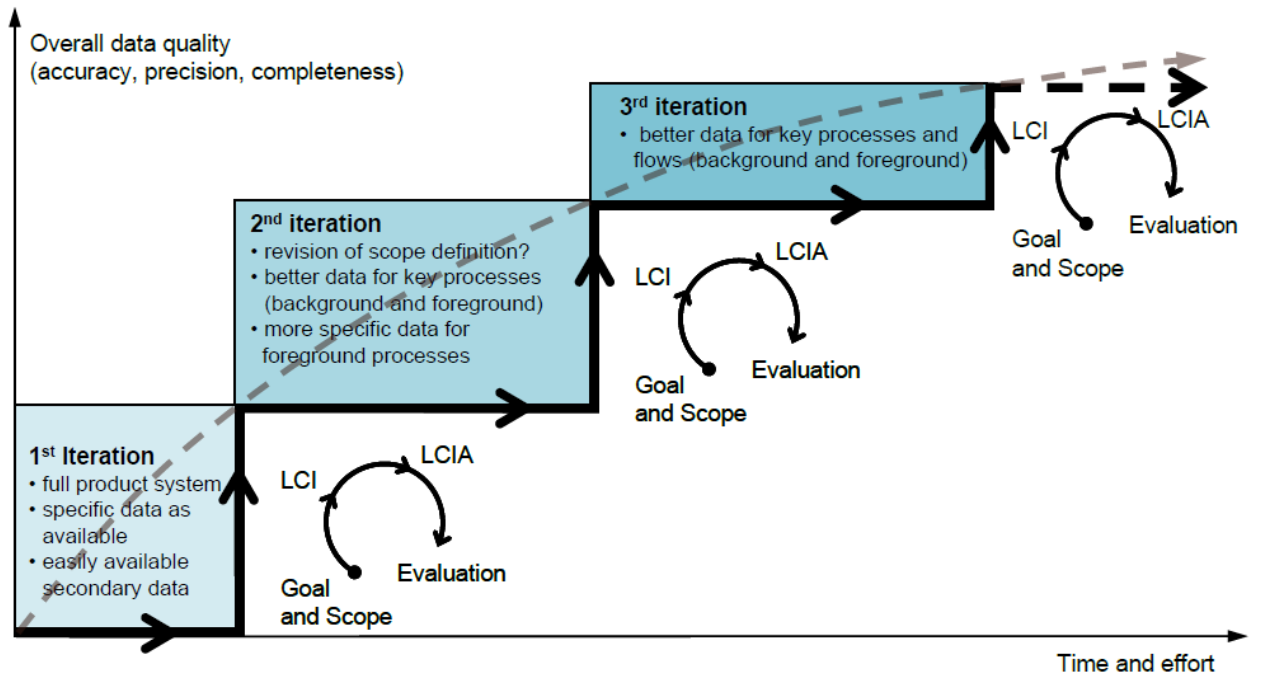
\includegraphics{image.png}
\caption{Data quality}
\end{figure}

\hypertarget{the-basics-of-life-cycle-inventory}{%
\subsection{The basics of life cycle
inventory}\label{the-basics-of-life-cycle-inventory}}

\begin{figure}
\centering
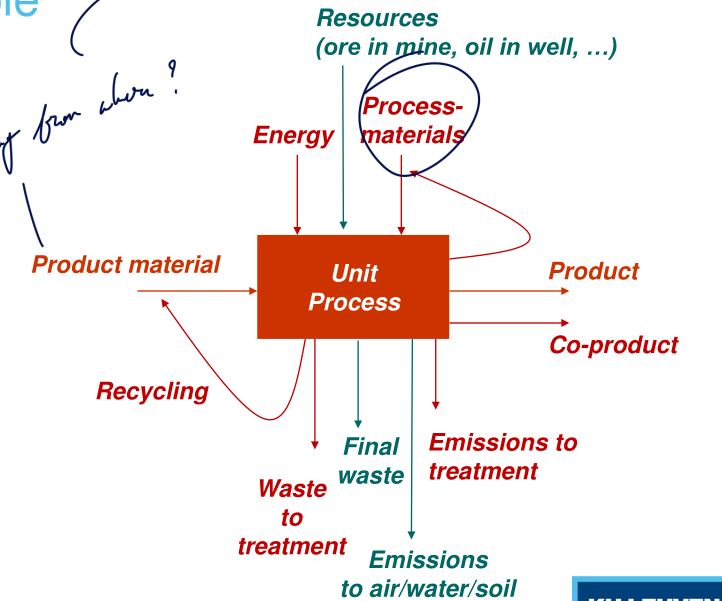
\includegraphics{image-1.png}
\caption{Principle of inventory}
\end{figure}

We need to analyze how much is going in and out, in emission but also
waste that can be further valorized sometimes. We also need to make the
distinction between the \emph{technosphere} and \emph{ecosphere}. When
talking about the ecosphere we are taking into account all the
ressources that comes from the nature while the technosphere takes into
account the economic flows of products and also waste.

We have the idea of \textbf{conservation of mass and energy}.

\begin{figure}
\centering
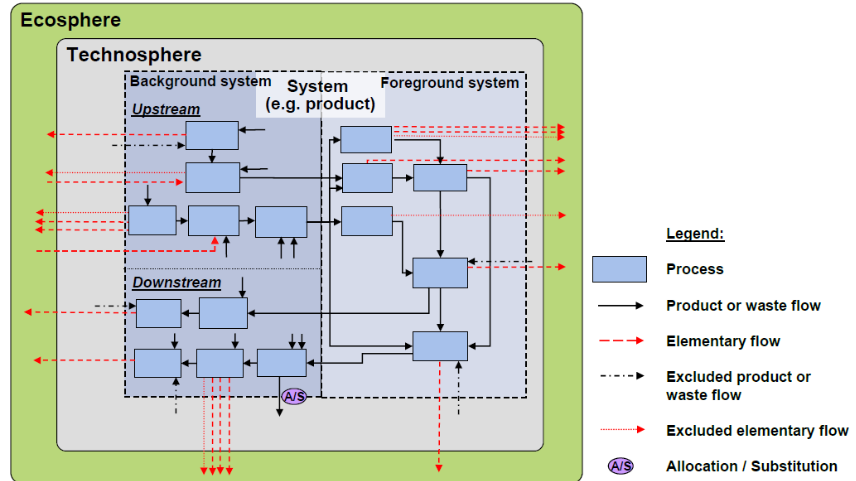
\includegraphics{image-2.png}
\caption{Typical analysis of flow}
\end{figure}

We have two types of processes

\begin{itemize}
\tightlist
\item
  Foreground : site specific data
\item
  Background : market averages
\end{itemize}

\hypertarget{multi-functionality}{%
\subsubsection{Multi-functionality}\label{multi-functionality}}

In most processes, we have some \emph{multi-functionality} since they
produces more than one \emph{functional flow}. For example we can
produce electricity and heat and use them both. We have various type of
multi-functionality :

\begin{enumerate}
\def\labelenumi{\arabic{enumi}.}
\tightlist
\item
  Co-production (multi-output)
\item
  Combined waste processing (multi-input)
\item
  Recycling (input-output)
\end{enumerate}

How to distribute the impacts of these processes ? That's the main
question we are trying to answer. We have 4 approaches that have their
strengths and weaknesses :

\begin{enumerate}
\def\labelenumi{\arabic{enumi}.}
\tightlist
\item
  More refined data over subdividing processes (can be expensive or not
  available)

  \begin{itemize}
  \tightlist
  \item
    Not partitioning but more refining of the data
  \end{itemize}
\item
  Partitioning (allocation)

  \begin{itemize}
  \tightlist
  \item
    We see the cost of producing the two products separately
  \item
    We need to reformulate our FU as a \emph{basket of products}. Not
    efficient when the processes are somewhere in the process tree.
  \item
    We are distributing the impact of something over an average load for
    example. We can't use those techniques for marginal things such as
    lightweight transport.
  \item
    Economic allocation

    \begin{itemize}
    \tightlist
    \item
      The economic incentive is a good way to partition. The price per
      kg can be tied with the consumption of functional flows.
    \item
      Can be hard to quantify with fluctuating prices, inflation, market
      distortions, not always disclosed prices
    \item
      Don't use it when \textbf{physical relationships} exist !
      Typically for products containing carbon we first have negative
      \(CO_2\) since we are taking the storage but then releasing it
      later.
    \end{itemize}
  \end{itemize}
\item
  System expansion

  \begin{itemize}
  \tightlist
  \item
    A bit like the partitioning instead we are looking just for the main
    product, never do for by-products or we will have flawed results. We
    need to set a determining product the first and main goal.
  \item
    Can have negative numbers.
  \item
    Implies that the other functional flows holds the impact of
    conventional production method (for new material production)
  \end{itemize}
\item
  Substitution

  \begin{itemize}
  \tightlist
  \item
    Always focus on the main driving and wanted production functional
    flow.
  \item
    Primarily used in \emph{consequential approach} but can be used for
    waste treatment in \emph{attributional studies}.
  \end{itemize}
\end{enumerate}

\begin{figure}
\centering
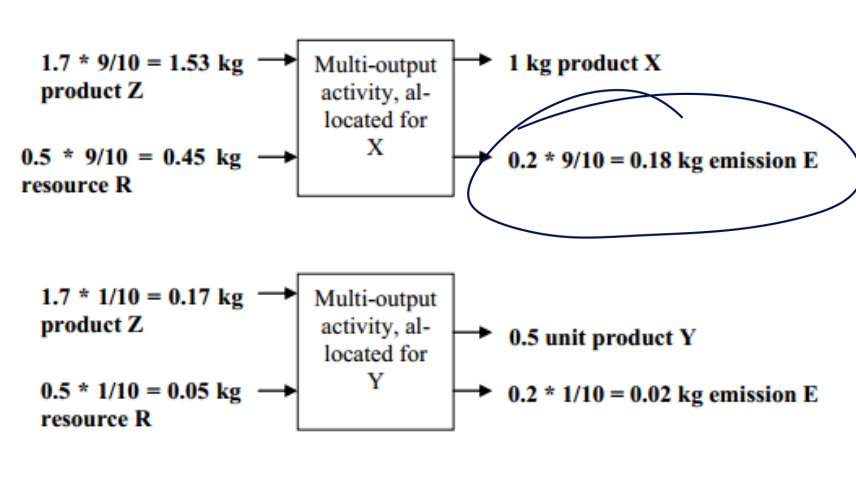
\includegraphics{image-3.png}
\caption{Partitioning}
\end{figure}

\begin{figure}
\centering
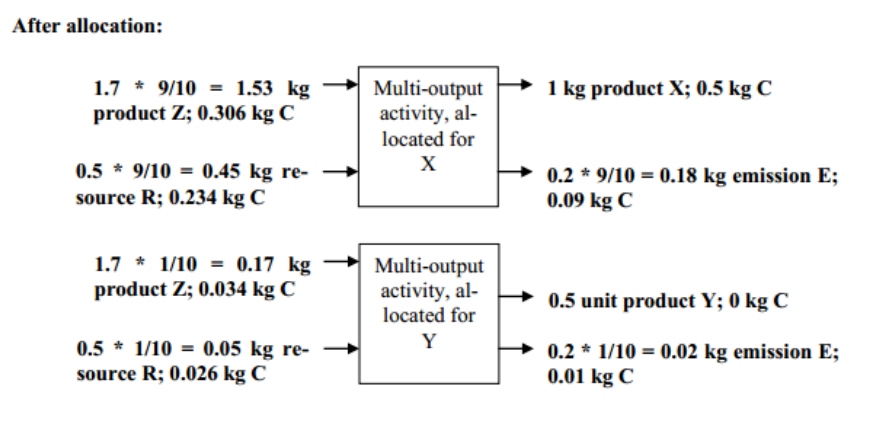
\includegraphics{image-4.png}
\caption{Bad partitioning when physical link exists}
\end{figure}

\hypertarget{allocation-at-point-of-substitution-apos}{%
\paragraph{Allocation at point of substitution
(APOS)}\label{allocation-at-point-of-substitution-apos}}

When we have waste, they can be valorized and transformed. But then we
need to take into account the market that is for this kind of product
and find the appropriate treating facilities. So we can see this process
as a black box but then we need to transform it so we can see the waste
as a product.

Sometimes it is best to simply do a cutoff if the by-products are
marginal in term of emissions and impacts.

Issues with our methods.

\begin{longtable}[]{@{}cc@{}}
\toprule\noalign{}
& problem \\
\midrule\noalign{}
\endhead
\bottomrule\noalign{}
\endlastfoot
system expansion & you don't answer the question you started with \\
substitution & which processes are avoided? \\
partitioning & what are the allocation factors? \\
\end{longtable}

``\emph{Allocation problem is artefact of wishing to isolate one
function. Artefacts can only be cured in an artificial way; there is no
``correct'' way, even not in theory}''

\hypertarget{marginal-vs-average}{%
\subsection{Marginal vs Average}\label{marginal-vs-average}}

Marginal is a sort of short term metric where we ask ourselves ``how
will X change if we stop doing this ?'' Usually it will lead to a stress
or a short term change on one specific sector.

But this can also lead to long term marginal where we dezoom and take a
closer look to change as a whole.

\hypertarget{modelling-approaches}{%
\subsection{2 modelling approaches}\label{modelling-approaches}}

\begin{longtable}[]{@{}
  >{\centering\arraybackslash}p{(\columnwidth - 4\tabcolsep) * \real{0.1942}}
  >{\centering\arraybackslash}p{(\columnwidth - 4\tabcolsep) * \real{0.4317}}
  >{\centering\arraybackslash}p{(\columnwidth - 4\tabcolsep) * \real{0.3741}}@{}}
\toprule\noalign{}
\begin{minipage}[b]{\linewidth}\centering
Specifications
\end{minipage} & \begin{minipage}[b]{\linewidth}\centering
Attributional approach
\end{minipage} & \begin{minipage}[b]{\linewidth}\centering
Consequential approach
\end{minipage} \\
\midrule\noalign{}
\endhead
\bottomrule\noalign{}
\endlastfoot
Description & Like book-keeping, we see the sum of impacts of all
products & Scenario analysis, calculated impacts reflect change \\
Data type & \textbf{average} & \textbf{marginal} \\
Solve multi-functionality ? & Partitioning and allocation & Substitution
(avoided products) \\
\end{longtable}

We need to be careful for the consequential approach as it uses
\emph{substitution}. We need to ask ourselves ``\emph{What is the
determining product ?}'', ``\emph{What is the avoided technology ?}''
(technology we are replacing with our innovation). Some new technology
can either add extra capacity to the market (\emph{increasing markets})
or simply force some old technology to shut down (\emph{decreasing
markets}). When we are looking short or long term it influences the
investment but not the \emph{capacity utilization}.

Constrained markets (regulated markets) are not marginal !

\hypertarget{modelling-context}{%
\subsubsection{Modelling context}\label{modelling-context}}

\begin{figure}
\centering
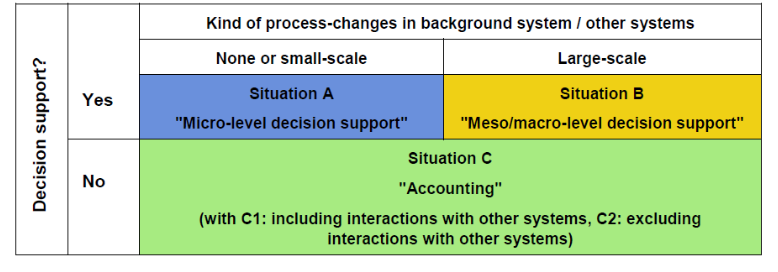
\includegraphics{image-5.png}
\caption{Modelling-context}
\end{figure}

\begin{itemize}
\tightlist
\item
  Ecoinvent advice for attributional

  \begin{itemize}
  \tightlist
  \item
    Studies at a societal level, where the entire environmental impact
    of all human activities is studied, with the aim of identifying
    areas for improvement
  \item
    Studies on environmental taxation, where the focus is less on the
    consequences of the tax, but rather on who is to carry the burden
  \item
    Studies that seek to avoid blame or to praise or reward for past
    good behavior
  \end{itemize}
\item
  Ecoinvent advice for consequential models:

  \begin{itemize}
  \tightlist
  \item
    Studies that investigate the long-term consequences(including
    changes in production capacity) of small-scale decisions (that don't
    change overall market conditions)
  \end{itemize}
\end{itemize}

\hypertarget{the-basics-of-life-cycle-impact-assessment}{%
\subsubsection{The basics of life cycle impact
assessment}\label{the-basics-of-life-cycle-impact-assessment}}

We have multiple steps :

\begin{itemize}
\tightlist
\item
  \textbf{Classification} : where does it contribute to ?

  \begin{itemize}
  \tightlist
  \item
    What is the contribution to global warming, acidification, \ldots{}
  \end{itemize}
\item
  \textbf{Characterization} : how much does it contribute ?

  \begin{itemize}
  \tightlist
  \item
    Put everything into \(CO_2\) equivalent. To have a common reference
  \end{itemize}
\item
  \textbf{Normalisation} : is this much ?

  \begin{itemize}
  \tightlist
  \item
    Normalize to the region, see how much contribution it is for europe,
    world, \ldots{}
  \end{itemize}
\item
  \textbf{Weighting} : is this important ?

  \begin{itemize}
  \tightlist
  \item
    Subjective step where we arbitrarily give more importance to
    specific part.
  \end{itemize}
\end{itemize}

We need to be careful with \emph{characterization} as it by itself
contains a certain weighting and choice. Namely, we only see the impact
of a given compound on a 100 year scale. So some molecules can be more
harmful on the short term but quickly degrade, this behavior won't be
seen in the \(CO_2\) equivalent methodology. Moreover, we can always
quantize this into a carbon footprint (human toxicity, eco-toxicity,
resource depletion). This is what we call the \textbf{mid-point}.

The \textbf{end-point} is more uncertain as we try to predict and
measure the impacts and possible scenarios. We also add the weighting
method to translate specific views \textbf{Individualist, Hierarchist
and Egalitarian}

\hypertarget{interpretation}{%
\subsubsection{Interpretation}\label{interpretation}}

We can :

\begin{enumerate}
\def\labelenumi{\arabic{enumi}.}
\tightlist
\item
  Draw conclusions
\item
  Sensitivity analysis
\item
  Report
\item
  Quality control (peer review)
\end{enumerate}

\hypertarget{input-output-lca}{%
\subsection{Input-output LCA}\label{input-output-lca}}

We need to put boundaries but it can be quite tricky to partition it.

\begin{figure}
\centering
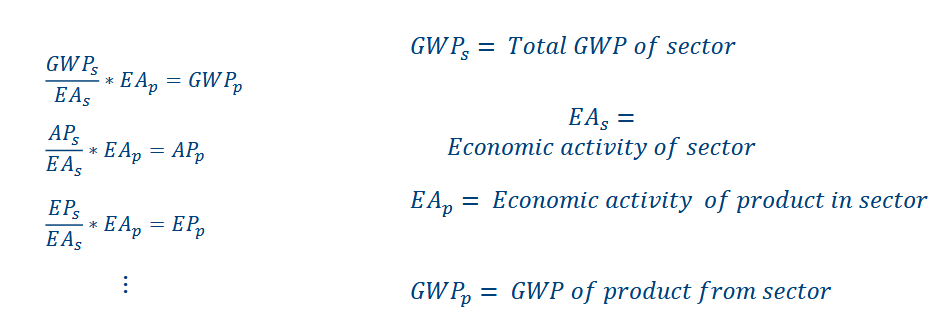
\includegraphics{image-6.png}
\caption{Partitioning}
\end{figure}

But it can be hard to measure and quantify the bi-directional
relationships that exists between all the sectors. We can build this IO
model based on the purchases between the sectors.

\begin{itemize}
\tightlist
\item
  Sum of Value Added (non-inter-industry purchases) and Final Demand is
  GDP.
\item
  Transactions include intermediate product purchases and row sum to
  Total Demand.
\item
  From the IO Transactions table, form the Technical Requirements matrix
  by dividing each column by total sector input -- matrix D. Entries
  represent direct inter-industry purchases per dollar of output.
\end{itemize}

With those tables we can create some matrices indicating the consumption
between the sectors.

\begin{figure}
\centering
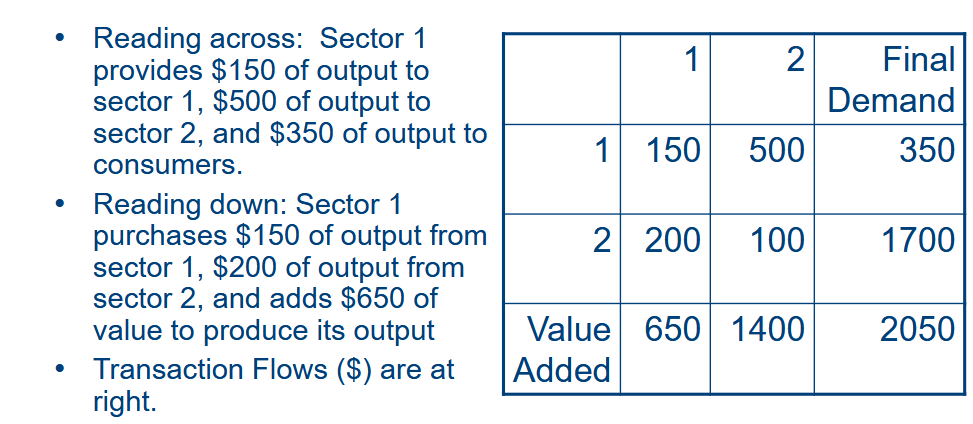
\includegraphics{image-7.png}
\caption{Example matrices}
\end{figure}

\begin{figure}
\centering
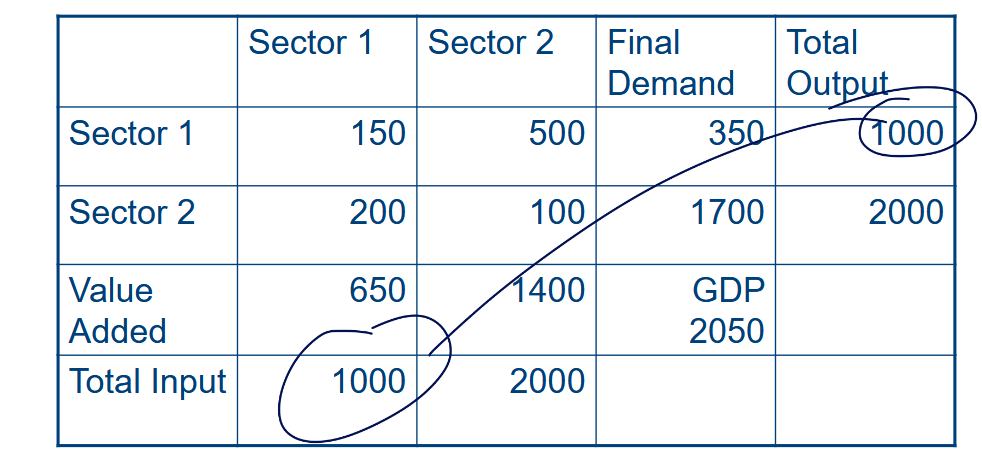
\includegraphics{image-8.png}
\caption{Final Matrix}
\end{figure}

\begin{longtable}[]{@{}
  >{\raggedright\arraybackslash}p{(\columnwidth - 8\tabcolsep) * \real{0.2366}}
  >{\raggedright\arraybackslash}p{(\columnwidth - 8\tabcolsep) * \real{0.1720}}
  >{\raggedright\arraybackslash}p{(\columnwidth - 8\tabcolsep) * \real{0.2473}}
  >{\raggedright\arraybackslash}p{(\columnwidth - 8\tabcolsep) * \real{0.1720}}
  >{\raggedright\arraybackslash}p{(\columnwidth - 8\tabcolsep) * \real{0.1720}}@{}}
\toprule\noalign{}
\begin{minipage}[b]{\linewidth}\raggedright
Output from sectors
\end{minipage} & \begin{minipage}[b]{\linewidth}\raggedright
Input to sectors
\end{minipage} & \begin{minipage}[b]{\linewidth}\raggedright
Intermediate output \(O\)
\end{minipage} & \begin{minipage}[b]{\linewidth}\raggedright
Final demand \(F\)
\end{minipage} & \begin{minipage}[b]{\linewidth}\raggedright
Total output \(X\)
\end{minipage} \\
\midrule\noalign{}
\endhead
\bottomrule\noalign{}
\endlastfoot
& 1 & 2 & 3 & n \\
1 & \(X_{11}\) & \(X_{12}\) & \(X_{13}\) & \(X_{1n}\) \\
2 & \(X_{21}\) & \(X_{22}\) & \(X_{23}\) & \(X_{2n}\) \\
3 & \(X_{31}\) & \(X_{32}\) & \(X_{33}\) & \(X_{3n}\) \\
n & \(X_{n1}\) & \(X_{n2}\) & \(X_{n3}\) & \(X_{nn}\) \\
Intermediate input \(I\) & \(I_1\) & \(I_2\) & \(I_3\) & \(I_n\) \\
Value added \(V\) & \(V_1\) & \(V_2\) & \(V_3\) & \(V_n\) \\
Total input \(X\) & \(X_1\) & \(X_2\) & \(X_3\) & \(X_n\) \\
\end{longtable}

\[
\sum X_{ij} + F_i = X_i \qquad \text{with } X_i = X_j \text{ and } A_{ij} = X_{ij}/X_j\\
\sum (A_{ij} X_j) + F_i = X_i\\
F = [I-A] X \quad X = [I-A]^{-1} F
\]

We normalize those matrix to have a view like ``how to make 1 € ?'' and
when building those matrices, we can even incorporate the additional
demand from a specific sector using \(X\). And with those simple
notation we can also quantify the environmental impact of various
production from different sectors.

\begin{figure}
\centering
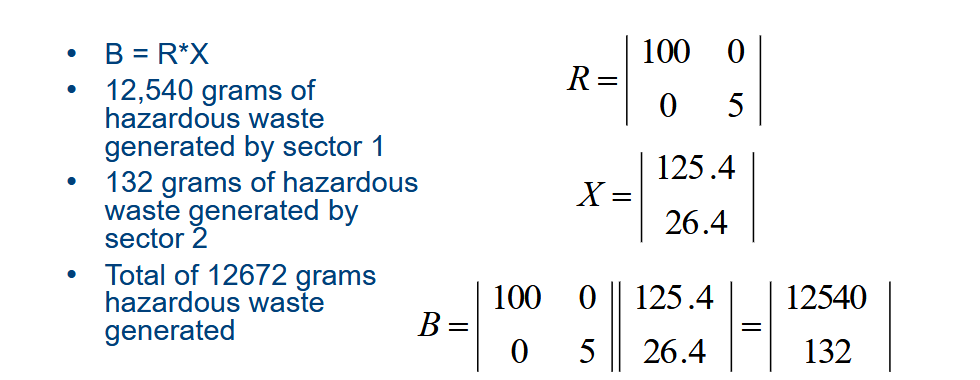
\includegraphics{image-9.png}
\caption{Hazardous}
\end{figure}

\hypertarget{design-for-environment-dfe-methods-and-techniques}{%
\section{Design for environment (DfE): Methods and
Techniques}\label{design-for-environment-dfe-methods-and-techniques}}

We want some fast, applicable methods that can be used in early design
phase that requires little additional expertise. So we can better design
for the environment.

\hypertarget{guidelines}{%
\paragraph{Guidelines}\label{guidelines}}

We have 5 requirements for sustainable products, the first 3 mimick the
protocols used by plant and animal ecosystems :

\begin{enumerate}
\def\labelenumi{\arabic{enumi}.}
\tightlist
\item
  \textbf{Cyclic:} the product is made form organic materials, and is
  recyclable or compostable, or is made form minerals that are
  continuously cycled in a closed loop
\end{enumerate}

\hypertarget{product-concept-optimisation}{%
\subsection{Product Concept
Optimisation}\label{product-concept-optimisation}}

test

\hypertarget{material-selection}{%
\subsection{Material Selection}\label{material-selection}}

test
